% !TeX spellcheck = en_US
% !TEX root = ../../phd.tex

\todo[inline]{shipments - Paper aktualsisieren}
\kmtTodo{Acronyme ersetzen}
\kmtTodo{e-trucks --> BEV}

Services vs Shipments als Grundlage für Nutzung kleinerer Fahrzeuge.

Rest aus Paper adaptiert übernehmen.

%\section{How Driving Multiple Tours Affects the Results of Last Mile Delivery Vehicle Routing Problems}
\label{el-shipments-...:sec}

\todo[inline]{Einleitung updaten/Umschreiben. ist noch von IK}
\textcolor{cyan}{In this chapter, an activity-based and dynamic approach is presented to analyze population
exposures to road traffic noise. The contribution of this innovative approach is that (1) affected
people at the workplace and places of education are incorporated and (2) the within-day dynamics
of varying population densities in different areas of the city is explicitly taken into account. The
proposed methodology is applied to a real-world case study of the Greater Berlin area.} 

This chapter is an edited version of a paper that has been previously published (\citet{MartinsTurnerNagel2019FreightMultipleToursABMTrans}).

\kmtTodo[inline]{Citation-commands mal ansehen. Cite sieht aus wie citet.}
\section{Introduction}
\label{sec:el-shipments-intro}
Urban freight transportation and last mile delivery are two major aspects of the growing e-commerce business. At the same time trucks are responsible for 35\% of \gls{co2}  emissions in Germany \citep{BMU2018KlimaschutzZahlen}. Recently, various courts have issued bans on diesel vehicles in various cities to protect the population from harmful emissions \citep{wikiDieselfahrverbot}. Additionally, environmentally-motivated measures to increase the quality of life are being discussed in society and politics\citep{SenStadt2013Luftreinhalteplan}. For investigating the effects of different measures it is important to have good simulation tools.  
Goods for a city typically arrive at distribution centers (``hubs'') at the periphery of the city, from where they need to be distributed further.  This implies solving a fleet assignment and \glspl{vrp}, so that each customer is included in a tour.  \Gls{jsprit} is an open source toolkit for solving such \glspl{vrp}.  It has been developed in conjunction with the transport planning software \acrshort{MATSim} (see below), but can also be used separately. \Gls{jsprit} can solve multi-depot problems, i.e.\ it does not only construct tours, but also assigns each destination to one of several hubs.  The approach is, however, not able to have the same vehicle perform multiple tours.  

In this paper, this is modified in a way that the vehicles can reload within the tours. This make it possible to reduce the number of vehicles needed for solving the problem and thus leads to a reduction of costs because fixed costs for some vehicles can be saved. This also brings the solution closer to reality, because companies want to have a high usage for their fleet. The investigation looks at the effects of reloading (and therefore running a second tour) compared to the previous situation of having only one tour per vehicle and day. For this, two different scenarios from two different sectors of urban commercial traffic are investigated.

%% Moced to Grundlagen - Modsim
%\paragraph*{Vehicle Routing Problem (VRP)}
%\label{vrp}
%\citet{IrnichEtAl2014VRP} define a \acrfull{vrp} as follows: Finding a plan to "determine a set of vehicle routes to perform [...] transportation requests with the given vehicle fleet at minimum costs"\cite{IrnichEtAl2014VRP}. A \gls{vrp} solves two interdependent main subproblems: (i) assigning requests to tours (clustering) and (ii) determining the optimal sequence in which the requests are served within a tour (routing).\cite{Prockl2010Informationsmanagement, Scheuerer2004HeuristikenTourenplanungPhd}
%
%The decision regarding optimal vehicle routing made by transport companies depends on various factors. Internal restrictions influencing the carrier can include the location of depot(s) and the available vehicle fleet at the depot(s). Each vehicle type has its own properties, e.g. capacity, fixed and variable costs and fuel consumption.
%External restrictions and specifications offer a framework in which carrier have to operate. Customer requests (quantity, type of good, location and time window to bring goods) are very important specifications for generating tour plans.\cite{JspritGithub} Further constraints such as driving restrictions and tolls can exist due to political or court decisions.\cite{Cerwenka2007Verkehrssystemplanung}
%The (expected) traffic situation has a direct impact on travel times. As a consequence, congestion can decrease service quality and can increase the costs of delivery for the carrier(s). Nevertheless, congestion is usually not considered in urban tour planning.\cite{Ehmke2012RoutingInCityLogistics} 
%For more information about different types for vehicle routing problems, see, e.g., \cite{TothVigo2014VRP}, \cite{Scheuerer2004HeuristikenTourenplanungPhd} or \cite{JspritGithub}.
%
%\paragraph*{jsprit}
%\label{jsprit}
%\Gls{jsprit} is an open source toolkit for solving \glspl{vrp}. For each \gls{vrp} there is a carrier which has a certain fleet and a list of requests. The fleet is located at the depot(s) from where they start and where they finish their tour. The fleet can be defined either by naming all available vehicles or by having an infinite fleet of defined vehicle type(s). When using the infinite fleet size, the composition of the fleet comes out as a result. The requests (or demand) can be defined in several ways: Either as \textit{service}s or as \textit{shipment}s. While services only have one location for delivering (or picking up) the goods - the other location is the depot - a shipment has two locations to define: from where to where the goods have to get transported. When applied to services, \gls{jsprit} can also solve \glspl{mdvrp}, which means that the algorithm also decides from which depot each request is served. \Gls{jsprit} iteratively optimizes the solution by ruining some parts of the solution and recreate a new one. 
%The aim of \gls{jsprit} is, to reduce the costs for the carrier. Costs can be e.g. fixed costs for the vehicle including depreciation, insurance, ..., variable cost for distance and time a vehicle is on tour, or other costs such as tolls or penalties for missed time windows.\cite{JspritGithub} 
%
%\paragraph*{Multi Agent-based Transport Simulation (MATSim)}
%\label{matsim}
%The \acrfull{MATSim} is an
%open source software for agent-based transport simulation. It is an activity-based, extendable framework implemented in Java, which is designed for large-scale scenarios. In addition to a common base, several optional extensions 
%are available (see \url{https://matsim.org/extensions}).\cite{MATSimBook}
%\gls{MATSim} is based on a co-evolutionary algorithm, where each iteration consists of the following three steps: Traffic simulation, scoring, and replanning. %(cf. Fig. \ref{fig:matsim}). 
%\gls{MATSim} simulates agents -- normally persons -- and their daily plans, which consist of activities like home or work and trips between their activity locations. These plans are simulated and then scored based on their experienced performance. After the scoring some agents try to improve their plans, e.g. by selecting a different route or modifying activity start and end times. For this, several strategies are available to generate new or modified plans. After this replanning step, a new iteration of the simulation starts with the modified plans. After running the specified number of iterations, \gls{MATSim} terminates after the scoring step.\cite{MATSimBook}
%
%\paragraph*{Freight traffic in MATSim}
%Simulating freight traffic in agent-based traffic simulations is often done similarly to usual passenger traffic. The drivers of the vehicles are the individual agents with fixed plans of their tour. Typically, they can only optimize their own route between the various destinations. An adjustment of the sequence within the tour is rarely performed, and moving pickups or deliveries from one agent/vehicle to another is not possible.\cite{ZilskeJoubert2015FreightTrafficInBook} Because of this one needs to generate the tour plans in advance. The already mentioned toolkit jsprit (see above) is a \gls{vrp} solver that is integrated into \gls{MATSim}. That integration is done by using the \gls{MATSim} freight contrib.\cite{ZilskeJoubert2015FreightTrafficInBook}

\vspace{-1mm} 
\section{Methodology}
\label{sec:el-shipments-methodology}
\vspace{-1mm} 
For enabling \gls{jsprit} to use vehicles for more than one tour and allow them to reload at the depot, the definition of the request is changed from service to shipment. 
As mentioned above, shipments have two locations (from and to) while services only have one (to or from -- depending if one looks at pickup or delivery) and the other one is always the depot. 
With shipments the vehicles can load or unload during their tour while with services the vehicles either start empty at the depot, pickup the request and return full to the depot or start full at the depot, deliver the requested goods and return empty. 
Solving service-based \glspl{vrp} needs far less computational time, because the capacity restriction of the vehicle does not need to be checked for every point within the tour. Converting a service-based \gls{vrp} to a shipment-based-\gls{vrp}  is very easy for \glspl{vrp} with only one depot: One only needs to add the depot as second location. 
For \acrfull{mdvrp} it is not clear from / to which depot the goods have to be delivered to which customer, because this is part of the \gls{vrp}. 
Because of that, first the service-based \gls{mdvrp} is solved -- which we also used here as a reference scenario. In a second step the shipments were created by looking up in the solution of the \gls{mdvrp}  where the tours with a certain request start, and set that as pickup location for the shipment.

\section{Scenarios}
\label{sec:el-shipments-scenarios}
The analysis of the effects of multiple tours are investigated in two different delivery scenarios located in the city of Berlin, Germany: (i) Food retailing in Berlin and (ii) Parcel delivery in Berlin-Wilmersdorf. They look at totally different sectors of commercial traffic. As a consequence, the underlying VRPs are different in the type and quantity of goods, vehicles that are used, etc. They were also originally set up from different teams and can therefore be used to get a better overview of the effects when enabling vehicles to run more than one tour.

\subsection{Food retailing scenario}
\label{sec:el-shipments-sceanrios-food} 
This scenario is based on the model of \citet{SchroederLiedtke2014FoodDistributionBerlin}. The effects of several urban freight measures were investigated in a case study of the food retailing industry in Berlin. It includes 1928 requests of 867 food retailing shops. The shops belong to 15 retailing companies in Berlin with 17 distribution centers in and around Berlin.
The shops' demand is the demand of an average day. Each shop has a variety of heterogeneous products they offer to their consumers, which require different transport conditions for supplying the shops. \citet{SchroederLiedtke2014FoodDistributionBerlin}  aggregated them into three different groups: fresh, frozen, and dry. 
This leads to $15 \, {\textit{companies}} \cdot 3 \frac{\textit{groups}}{\textit{company}} = 45 \, {\textit{carriers}}$ in the model, that is, ``fresh'', ``frozen'' and ``dry'' are transported by different carriers. Each carrier has its own fleet available. The available vehicle types in the fleet of a carrier depend on the group type of goods and the business type of the company. Some retailing companies have more than one depot for supplying their shops.

\paragraph*{Scenario description}
In the \textbf{reference scenario (single tour)} the capabilities for the three different product groups were set as they were defined by \citet{SchroederLiedtke2014FoodDistributionBerlin}:

\begin{itemize}[]
\item \textbf{Fresh} products are delivered in a time-window of [4am -- 9am].
\item \textbf{Frozen} and {dry} products are delivered either in a time-window of [9am -- 2pm] (``morning'') or [2pm -- 7pm] (``afternoon'').  For each delivery, the time-window is randomly assigned.
\end{itemize}

In this model, the demand of the different stores is represented by the activity type "service". As mentioned in Sec.~\ref{sec:gl-modsim-vrp-jsprit}, it is possible to model it as an \gls{mdvrp}, but  then each vehicle only drives one tour from the depot to its customers and returns to the depot. 
In consequence there are many more vehicles needed than necessary for supplying all shops.
Note that it is not possible to ``re-use'' vehicles: A vehicle that was used for dry products between 9am and 2pm cannot be re-used between 2pm and 7pm.
Because of the underlying cost model with fixed costs for each employed vehicle this leads to an inefficient solution with too high costs \citep{MartinsTurnerNagel2019FreightMultipleToursABMTrans}.

\citet{MartinsTurnerNagel2019FreightMultipleToursABMTrans} investigated several policies, which in part reinvestigate previous results \citep{SchroederLiedtke2014FoodDistributionBerlin}, and by introducing city hubs (called \Glspl{ucc}) went beyond. 
The policy measures with respect to the existing \acrfull{lez} of Berlin were:

\begin{itemize}
\item (A1) Cordon toll (20 \euro{}) for heavy diesel trucks (26t or 40t) for entering the \gls{lez}
\item (A2) Cordon toll (20 \euro{}) for heavy diesel trucks (26t or 40t) for entering the\gls{lez}, e-trucks available at depots
\item (B) Prohibition of diesel trucks inside the \gls{lez}, e-trucks available at depots
\item (C) Prohibition of diesel trucks inside the \gls{lez}, e-trucks available at depots, and three \gls{ucc} inserted close to the \gls{lez} to supply the shops within the \gls{lez}with e-trucks. The city hubs were supplied from the main depots.
\end{itemize}


For the \textbf{improved algorithm} (vehicles can do multiple tours), it is no longer necessary to have two separate shifts for having tours in the afternoon. As a consequence, the time windows for delivering as well as the availability of vehicles at the depots for frozen and dry goods were combined into one single time window of [9am -- 7pm]. The time window of [4am -- 9am] for fresh goods remain unmodified, because fresh goods should be available in the stores in the morning. Note that the ``fresh goods'' vehicles cannot be re-used for ``dry'' or ``frozen'' goods, since they belong to a different carrier. Now the algorithm can choose which shops are supplied when. All policies remain the same as in the reference (single-tour) scenario. 

\vspace{-2mm} 
\paragraph*{Results}
Comparing the results (single tour vs multiple tours) for the different cases, one can see that allowing vehicles to drive several tours leads to the expected results (see Fig. \ref{fig:BerlinFoodSinglevsMultiTours} and Tab. \ref{tab:BerlinFoodSinglevsMultiToursData}). The number of vehicles used decreases by approx. 62.5 $-$ 68 \% depending on the investigated policy. Due to the high influence of fixed costs savings when running only one tour per vehicle, the costs now decrease by 35 - 44 \%. The distance travelled and travel time slightly decrease by up to 6\%. The consumption of diesel and therefore the \gls{co2} emissions increase by up to 3.8 \%. 

\begin{figure}[t]%\vspace*{4pt}
\begin{minipage}[t]{0.45\textwidth}
\centerline{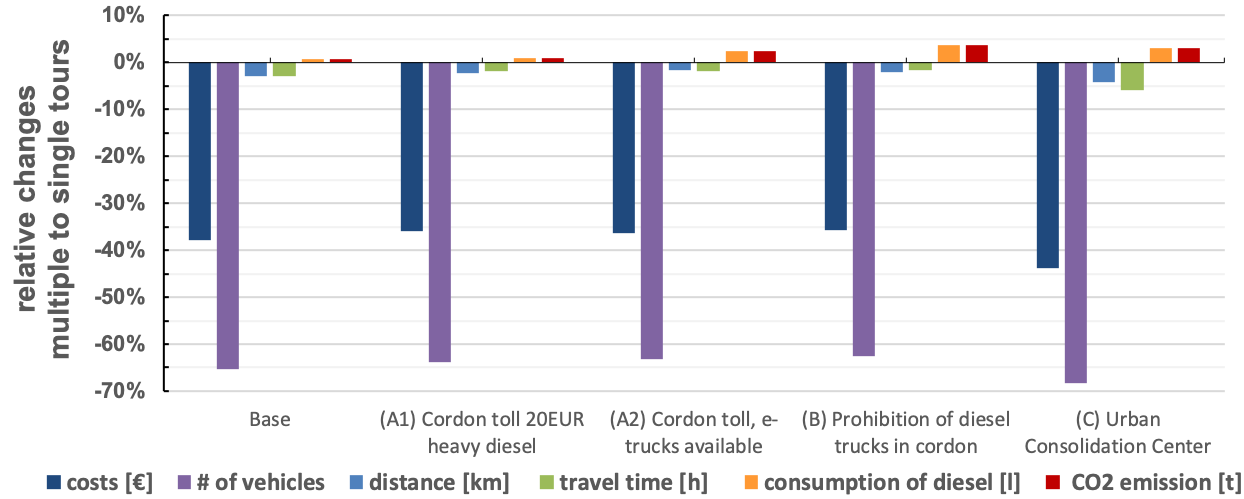
\includegraphics[width=0.9\textwidth]{elektrifizierung/shipments/figs/BerlinFoodSinglevsMultiTours}}
\caption{Comparison of results for all cases when vehicle can run more than one tour (improved algorithm) instead of only one tour}
\label{fig:BerlinFoodSinglevsMultiTours}
\end{minipage}
\hspace{0.05\textwidth}
\begin{minipage}[t]{0.45\textwidth}
\centerline{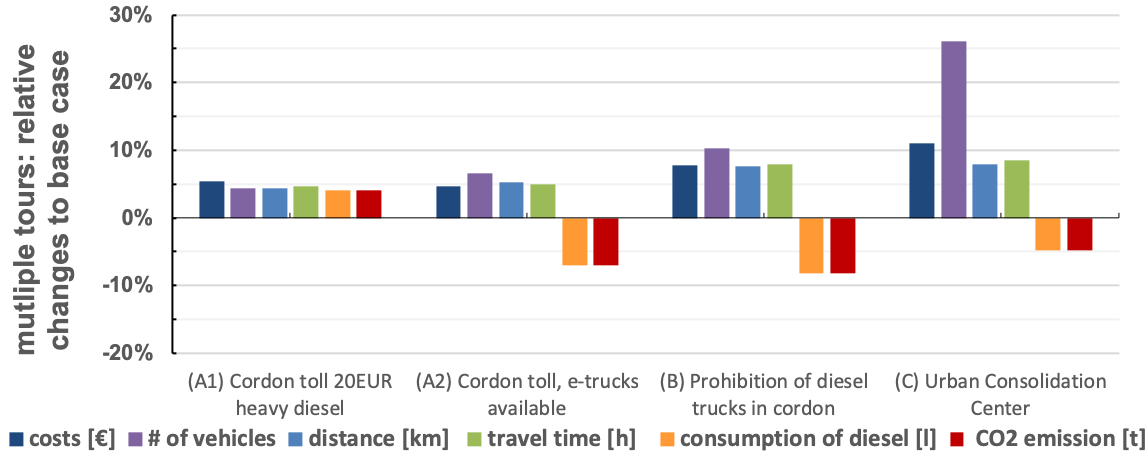
\includegraphics[width=\textwidth]{elektrifizierung/shipments/figs/BerlinFoodMultipleTours}}
\caption{Relative changes compared to the base case when using the improved algorithm (vehicles can do multiple tours)}\vspace*{-6pt}
\label{fig:FoodMutlipleTours}
\end{minipage}
\vspace{-5mm} 
\end{figure}

\kmtTodo{Tabellen sind am Ende des Chapters... wie kommen die an die richtige Stelle}
\kmtTodo{Tabellen sind zu breit}
\begin{table}[b]
\vspace{-3mm} 
\caption{Comparison of results when vehicle can run \textit{more than one tour} (m) instead of only one single tour (s) for Berlin food retailing scenario}
\begin{tabular*}{\hsize}{@{\extracolsep{\fill}}llrrrrrr@{}}
\toprule
policy &  algorithm & costs (\euro) & \# of veh. & distance (km) & travel time (h) & fuel (l) & \gls{co2}  (t)\\
\midrule
\multirow{ 3}{150pt}{Base} & s &  114,575 &  529 & 38,146 & 706.8 & 11,170 & 29.3 \\
& \textit{m} & \textit{71,263} & \textit{184} & \textit{37,072} & \textit{686.4} & \textit{11,254} & \textit{29.5 }\\ 
& \textbf{diff.} & \textbf{ $-$ 43,313} & \textbf{ $-$ 345} &  \textbf{$-$ 1,704} &  \textbf{$-$ 20.4} & \textbf{+ 84} & \textbf{+ 0.2}\\ \hline
 
\multirow{ 3}{150pt}{(A1) Cordon toll 20EUR heavy diesel}  & s &  117,391 &  532 & 39,614 & 732.5 & 11,612 & 30.4\\
& \textit{m} &  \textit{75,120} & \textit{192} & \textit{38,682} & \textit{718.9} & \textit{11,721} & \textit{30.7} \\ 
& \textbf{diff.} & \textbf{$-$ 42,271} & \textbf{$-$ 340} &  \textbf{$-$ 932} &  \textbf{$-$ 13.6} &  \textbf{+ 109} & \textbf{+ 0.3} \\ \hline

\multirow{ 3}{150pt}{(A2) Cordon toll, e-trucks available} & s &  117,345 &  534 & 39,683 & 733.4 & 10,229 & 26.8\\
& \textit{m} & \textit{ 74,637} & \textit{196} & \textit{39,051} & \textit{720.4} & \textit{10,470} & \textit{27.4}\\ 
& \textbf{diff.} & \textbf{ $-$ 42,708} & \textbf{$-$ 338} &  \textbf{$-$ 632} &  \textbf{$-$ 13.0} & \textbf{+ 241} & \textbf{+ 0.6}\\ \hline

\multirow{ 3}{150pt}{(B) Prohibition of diesel trucks in cordon, e-trucks available} & s & 119,552 &  542 & 40,707 & 753.7 & 9,951 & 26.1\\
& \textit{m} & \textit{76,842} & \textit{203} & \textit{39,907} & \textit{741.3} & \textit{10,328} & \textit{27.1}\\
& \textbf{diff.} & \textbf{$-$ 42,710} & \textbf{$-$ 339} &  \textbf{$-$ 800} &  \textbf{$-$ 12.4} & \textbf{+ 377} & \textbf{+ 1.0}\\ \hline

\multirow{ 3}{150pt}{(C) Urban Consolidation Center} & s & 140,891 &  731 & 41,805 & 791.7 & 10,401 & 27.3\\
& \textit{m} & \textit{79,083} & \textit{232} & \textit{40,036} & \textit{744.7} & \textit{10,715} & \textit{28.1}\\ 
& \textbf{diff.} & \textbf{$-$ 61,808} & \textbf{$-$ 499} &  \textbf{$-$ 1,769} &  \textbf{$-$ 47.1} & \textbf{+ 314} & \textbf{+ 0.8}\\
\bottomrule

\end{tabular*}
\label{tab:BerlinFoodSinglevsMultiToursData}
%%\vspace{-3mm} 
\end{table}

The effects of the policy cases compared to the base case of the policy (multiple tour) scenario (see Fig. \ref{fig:FoodMutlipleTours}) go in the same direction as in the reference (single tour) scenario. But the relative changes are -- except for the changes in number of vehicles used -- approximately the same. For the \gls{ucc} case a significantly lower increase of costs and vehicles used were observed. This arises from the intended more-efficient usage of the vehicles.

\subsection{Parcel delivery Berlin-Wilmersdorf}
\label{sec:el-shipments-kep}
\nopagebreak
\paragraph*{Scenario description}
The subject of this scenarios is the last mile parcel delivery of an average day in one district of Berlin. 
As the main data for this case two scenarios, with 1,217 requests with the demand of 1..12 parcel(s) each, from \citet{ZhangEtAl2018UrbanParcelDelivery} were considered:
(scenario 1) Distribution of all parcels directly from the (one) \gls{DC} by light parcel delivery trucks, and
(scenario 2) Commercial parcels are firstly delivered from the \gls{DC} to given micro depots by light parcel delivery trucks and from there delivered to the customers by cargo bicycles. Parcels to private recipients are still directly delivered by cargo vehicles from the DC.

For both scenarios, two simulations were also run. One service-based (reference scenarios: only one tour per vehicle per day) and one shipment-based (policy scenarios: vehicles can reload within the tour). In contrast to the food retailing scenario, for the \textbf{improved algorithm} an adaption of the time-windows for delivery and vehicle availability was not necessary, because no manual shifts were defined by \citet{ZhangEtAl2018UrbanParcelDelivery}. 

\paragraph*{Results}
For scenario 1 (direct delivery) the improved algorithm ($=$ multiple tours per vehicle) did not lead to a significantly different result in terms of costs, distance, time, ... (see Tab. \ref{tab:CEP1SinglevsMultiToursData}). It just seems to be another heuristic solution as it was seen in the service-based \gls{vrp} ($=$ one tour per vehicle), but no change due to the modification to a shipment-based. Even with the improved algorithm none of the 20 vehicles reload during the day.
This makes sense, because the restriction in this case was the time window (9am -- 5/6pm) and not the capacity of the vehicles. Because of this, enabling reloading has no positive influence on the fleet sizes needed. 

\kmtTodo{Tabellen sind am Ende des Chapters... wie kommen die an die richtige Stelle}
\kmtTodo{Tabellen sind zu breit}
\begin{table}[tb]
%\vspace{-3.5mm} 
\caption{Comparison of results when vehicle can run \textit{more than one tour (m)} instead of only one tour (s) for CEP scenario 1 (direct distribution)}
\begin{tabular*}{\hsize}{@{\extracolsep{\fill}}lllrrrrrr@{}}
\toprule
policy & algorithm & costs (\euro)  & \# of vehicles & distance (km) & travel time (h) & fuel consumption (l) & \gls{co2}  (t)\\
\midrule
\multirow{ 3}{50pt}{scenario 1: direct distribution} & s  &  6,066  & 21 & 237.3 & 10.75 & 26.58 & 7.12 \\
& \textit{m}  & \textit{5,938} & \textit{20} & \textit{259.3} & \textit{11.96} & \textit{29.04} & \textit{7.78}\\ 
& \textbf{diff.} & \textbf{$-$ 128} & \textbf{$-$ 1} & \textbf{+ 22.0} & \textbf{+ 1.21} & \textbf{+ 2.46} & \textbf{+ 0.66}\\ 
\bottomrule
\end{tabular*}
\label{tab:CEP1SinglevsMultiToursData}
%\vspace{-4mm} 
\end{table}

In addition to the stated results, a very large increase in computation time was observed for this scenario. Solving the service-based \gls{vrp} took less than 1.5 hours, while the shipment-based \gls{vrp} ran for several days until the algorithm terminated. This is dramatically longer than it was observed in the food retailing scenario above and seems to be related to the significantly larger number of shipments. 

For scenario 2, with micro depots and cargo bicycle delivery for the last mile, the multiple tour algorithm significantly reduces the number of vehicles and therefore costs (see Tab. \ref{tab:CEP2SinglevsMultiToursData}). This is expected because of the significantly lower capacity of the cargo bicycles, so the tours in the single run case were restricted by the capacity limit and not by temporal availability. In this scenario, the number of light parcel delivery trucks used decrease as well, because they have shorter tours with higher demand to deliver the commercial parcels to the micro depots and the private parcels directly to the recipients.

\kmtTodo{Tabellen sind am Ende des Chapters... wie kommen die an die richtige Stelle}
\kmtTodo{Tabellen sind zu breit}
\begin{table}[b]
%\vspace{-3.5mm} 
\caption{Comparison of results when vehicle can run \textit{more than one tour} (m) instead of only one tour (s) for CEP scenario 2 (micro depots and cargo bicycles for commercial parcels)}
\begin{tabular*}{\hsize}{@{\extracolsep{\fill}}lllrrrrrr@{}}
\toprule
policy &  algorithm & vehicle type & costs (\euro)  & \# of vehicles & distance (km) & travel time (h) & fuel consumption (l) & \gls{co2}  (t)\\
\midrule
\multirow{ 9}{50pt}{scenario 2:  micro depots} & \multirow{3}{*}{s} & total  &  7,056 &  141 & 650.5 &	30.86 & 19.86 & 5.32 \\
&& cargo bicycle & & 121 & 473.2 &	21.79 &  0 & 0\\
&& parcel truck & & 20 & 177.3 & 7.91 & 19.86 & 5.32\\

\cline{2-9}

& \multirow{3}{*}{\textit{m}} & \textit{total} & \textit{6,396}  & \textit{45} & \textit{690.3} & \textit{30.86} & \textit{20.01} & \textit{5.36}\\ 
&& \textit{cargo bicycle} & & \textit{33} & \textit{511.6} & \textit{22.95} & \textit{0} & \textit{0}\\ 
&& \textit{parcel truck} & & \textit{12} & \textit{178.7} & \textit{7.91} & \textit{20.01} & \textit{5.36}\\ 

\cline{2-9}

& \multirow{3}{*}{\textbf{diff.}} & \textbf{total} & \textbf{$-$ 660}  & \textbf{$-$ 96} & \textbf{+ 39.8} & \textbf{+ 1.16} & \textbf{+ 0.15} & \textbf{+ 0.04}\\ 
&& \textbf{cargo bicycle} & & \textbf{$-$ 88} & \textbf{+ 38.4} & \textbf{+ 1.16} & \textbf{0} & \textbf{0}\\ 
&& \textbf{parcel truck} & & \textbf{$-$ 8} & \textbf{+ 1.4} & \textbf{ 0} & \textbf{+ 0.15} & \textbf{+ 0.04}\\

\bottomrule
\end{tabular*}
\label{tab:CEP2SinglevsMultiToursData}
%\vspace{-4mm} 
\end{table}

%\vspace{-1mm} 
\section{Conclusion}
\label{sec:el-shipments-conclusion}
%\vspace{-1mm} 
In this article an enhancement of solutions for tour planning problems has been presented. It demonstrates the high influence of eliminating tour planning restrictions for the solution of \glspl{vrp}. 
Allowing the algorithm to use vehicles for more than one \textit{depot - customer - ... - customer - depot} tour per day reduces the fleet size by about 2/3 for the cases of food retailing and parcel delivery by cargo bicycles from micro hubs. The costs decreases, dependent on the case, by about 9 to 44 \%. 
If the vehicle capacity is not the deciding restriction, no significant reduction of the fleet size (and costs) can be observed.
In all scenarios, only small changes in distance, time traveled, fuel consumption and therefore the \gls{co2}  emissions by the whole fleet were observed.

For our investigations we improved the collaboration of the agent-based transport simulation software MATSim and the vehicle routing problem solver jsprit. Using \textit{shipments} instead of \textit{services} allows the algorithm to reload at the depot and continue with the current vehicle. Allowing the algorithm to use vehicles for more than one tour allows to break up the implicitly given separation of delivering shifts. For evaluating the effects, two independent scenarios were used. The first is about supplying food retailing shops in Berlin. The second scenario is about parcel delivery in one district of Berlin. Both scenarios have different designs and policy cases to see the effects under different situations. 

Using the proposed approach for multi-depot VRPs (MDVRP) means that one has to run jsprit twice: First as a {MDVRP} with the computationally faster and multi-depot-able activity type \textit{service}. From the tour plan the "shipment"-based VRP is generated which can go into the second, computationally slower but multi-tours-capable \textit{shipment-}based jsprit run. This double running one VRP also has the effect that the assignment of a request to a certain depot is maybe not optimal for the run with multiple tours. The increase of computation time for the shipment-based VRPs is in an acceptable range for VRPs with up to approx. 200 shipments per carrier. In the CEP scenario 1, with more than 1200 shipments for one single carrier, the computational time increases from less than 1.5 hours to four days.

%\kmtTodo{remove acknowledgment?}
%\section*{Acknowledgements}
%This work was supported by the DFG (Deutsche Forschungsgemeinschaft - German Research Foundation) under the grant 323900421. We thank Stefan Schröder and Gernot Liedtke for providing their data of the Berlin food retailing scenario. We also thank Lei Zhang, Tilman Matteis, Carina Thaller and Gernot Liedtke for providing their data of the Berlin-Wilmersdorf CEP scenario.


%%%%%%%%%%%%%%%%%%%%%%%%%%%%
%%%%%%%%%%%%%%%%%%%%%%%%%%%%
